\chapter{JDart et exécution concolique}
  \paragraph{}
    L'idée générale est de rendre la tâche de tester des Applets Java Card moins penible et plus effective que possible.
    Pour celà nous optons pour l'utilisation de l'execution concolique comme une technique d'analyse ce qui permet de rendre 
    le system à tester moins obscue et plus predictible surtout quand on est face à des systemes complexe
    et qui nécessite des méthodes plus avancées qu'un simple teste unitaire.
  \paragraph{}
    JDart est un outil qui permet d'utiliser l'execution concolique comme une technique pour tester les applications Java.
    \newline
    JDart est une extension de \gls{JPF} un outil créé par le NASA afin de tester ses applications y compris les programmes executés sur ses robots astromobiles.
  \section{Exploration des chemins et l'execution concolique}
    \paragraph{Java Path Finder: Exploration des chemins}
      \gls{JPF} est un outil de verification du modéle d'état pour le bytecode Java,
      ce qui rent \gls{JPF} est en fait une \gls{VM} qui execute le programme donné en entrée autant de fois que nécessaire
      afin d'explorer chaque chemin qu'il contient.
      Tout au long de ce processus, \gls{JPF} collecte les anomalies rencontrés tel que l'interblocage des threads ou des exceptions non traités puis
      il génére un rapport contenant les traces qui méne à ces anomalies.
      \begin{figure}
	\centering
	  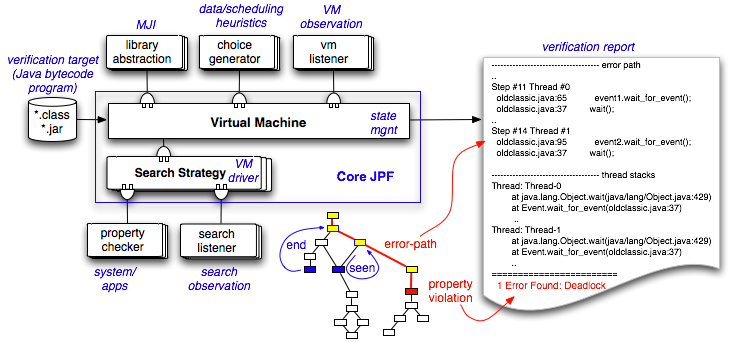
\includegraphics[width=1\textwidth]{images/jpf-model.png}
	\caption{modéle d'opération de \gls{JPF}}
      \end{figure}
  \section{La VM JAVA, La VM du JPF et la JavaCard VM}
  \section{Tester des applets JavaCard}
  \paragraph{}
    Java Path Finder connu comme le couteau Suisse de la verification Java,
    est en effet un des outis de teste les plus evolués pour les applications Java,
    grâce à son extensibilité et à son abilité de supporter et interger de nouvelle extensions.
    Cependant, la majorité des extensions ne sont pas destinés à être executer sur des systemes Java Card.